\documentclass[twocolumn,amsmath,amssymb,aps]{revtex4}
\usepackage{graphicx}% Include figure files
\usepackage{dcolumn}% Align table columns on decimal point
\usepackage{bm}% bold math
\usepackage{color, subfigure}

\begin{document}
\title{An Overview of a Realistic Model for the Belousov-Zhabotinsky Reaction}%
\author{Huan Q, Bui}\email{hqbui21@colby.edu}
\affiliation{Departent of Physics and Astronomy, Colby College.}
\date{\today}
\begin{abstract}
This paper reviews the Oregonator, a realistic, mathematical model for chemical oscillations, of which the Belousov-Zhabotinsky reaction is a prime example. Extensively discussed therein are descriptions of how the Oregonator captures the characteristic behaviors of the Belousov-Zhabotinsky reaction through the existence of limit cycles and excitability. The paper also covers experimental data to illustrate how these mathematical aspects manifest in a real reaction. 
\end{abstract}
\maketitle




\section{Introduction}
The Belousov-Zhabotinsky (BZ) reaction, named after Soviet chemists Boris Belousov (1893 - 1970) and Anatol Zhabotinsky (1938 - 2007), is among a large class of chemical oscillators. The reaction was first discovered by Belousov in 1951 in his attempt to mimic glycolysis, an oscillatory biochemical process. Using a mixture of potassium bromate, cerium(IV), sulfate, malonic acid, and citric acid in dilute sulfuric acid at appropriate proportions, Belousov found that the solution in which the reaction took place spontaneously oscillated in color between clear and yellow rather than reaching an equilibrium state. This behavior was so peculiar that Belousov's contemporaries were reluctant to publish his results, citing an apparent violation of the second law of thermodynamics \cite{ball1999self}. Belousov ultimately managed to publish his results, though in a less reputed and non-peer-reviewed journal. In 1961, the reaction was further studied by Zhabotinsky and only gained popularity following a conference in Prague in 1968 \cite{doi:10.1021/ed061p661}.

The BZ reaction remains popular to this day both in and outside the academic circles. It is a prime example for a nonlinear system which exhibits excitability and oscillatory behaviors. Following its emergence, building mathematical models for the reaction also attracted significant interest. Most notable examples of these models are the \textit{Brusselator}, proposed by Ilya Prigogine and his collaborators at the Université Libre de Bruxelles, and the \textit{Oregonator}, proposed by Richard Field and Richard M. Noyes at the University of Oregon. While the Brusselator helped motivate interest in chemical pattern formation, it does not model a realistic BZ reaction. The Oregonator, on the other hand, captures many aspects of a true chemical oscillator including limit cycle dynamics and excitability. In the following sections, we will explore the dynamics captured by the Oregonator via numerical simulations in MATLAB. 
\section{The Oregonator}
The Oregonator is a system of two coupled ordinary differential equations \cite{doi:10.1063/1.1681288}:
\begin{eqnarray*}
\epsilon \dot{U} &=& U(1-U) - fV(U-q)/(U+q) \\
\dot{V} &=&  U-V
\end{eqnarray*}
where $U,V$ represent the concentrations of chemical reactants and $(f,q,\epsilon)$ are the model parameters. The equilibrium concentrations are attained whenever $\dot{U} = \dot{V} = 0$. These solutions are given by the following expressions:
\begin{eqnarray*}
U_{\text{eq}} &=& \frac{1}{2}\left[1-q-f + \sqrt{(1-q-f)^2 + 4q(1+f)}\right]\nonumber \\ 
V_{\text{eq}} &=& U_{\text{eq}}. 
\end{eqnarray*}
One finds this equilibrium solution by intersecting the nullclines $\dot{U} = 0$ and $\dot{V} = 0$:
\begin{eqnarray*} 
V &=& \frac{U(1-U)(U+q)}{f(U-q)}\\
V &=&U 
\end{eqnarray*}
It is clear that the first nullcline depends only on the parameters $f$ and $q$, and the second nullcline is independent of all model parameters. For the rest of this paper, we will assume $q$ is fixed unless stated otherwise. As we will see later, by varying $f$, the model exhibits markedly different behaviors. 

\subsection{Limit Cycle}
The Oregonator captures the oscillatory behavior of the BZ reaction through the existence of the \textit{limit cycle} for certain combinations of the parameters $f,q$, and $\epsilon$. A limit cycle is an attractor, i.e., a solution for the Oregonator towards which the system tends to evolve in the large-time limit. The limit cycle shows up as a closed trajectory in phase space. In the presence of a limit cycle, no out-of-equilibrium state of the system converges to the equilibrium state.

\begin{figure}[!htb]
	\includegraphics[scale=0.5]{limit_cycle_f_065_e_1e-2.eps}
	\caption{Limit cycle (black) and nullclines (blue), for $f = 0.65, \epsilon = 10^{-2}, q = 0.002$. All trajectories (except for the equilibrium trajectory) converge to the limit cycle, including points near the equilibrium solution. Points to left of the $V=U$ nullcline converge the limit cycle from the right, and vice versa. The system does not converge to  a fixed point.}
	\label{fig:LC}
\end{figure}

Figure \ref{fig:LC} shows the phase portrait of the system at $f = 0.65, \epsilon = 10^{-2}$, and $q = 0.002$, at which a limit cycle is present. It is clear that all phase trajectories, except for the equilibrium trajectory at $U_{\text{eq}} = V_{\text{eq}} = 0.3572$ (which is the intersection between two nullclines highlighted in blue), converge to the counter-clockwise limit cycle highlighted in black. All trajectories which begin below the curved nullcline first evolve towards an increase in $U$, while those above this nullcline first evolve towards a depletion in $U$. Figure \ref{fig:UVTime} illustrates how the system evolves following the initial condition given by $U_0 = 0.2, V_0 = 0.26$, which is above the curved nullcline. 


\begin{figure}[!htb]
	\centering
	\includegraphics[scale=0.5]{UV_Time.eps}
	\caption{Oscillations in concentration of $U,V$ in time is the presence of a limit cycle. The system evolves from the initial condition $U_0 = 0.2, V_0 = 0.26$}
	\label{fig:UVTime}
\end{figure}


Just to emphasize the fact that \textit{all} trajectories, no matter how close to the equilibrium solution, converge the limit cycle, we consider the initial condition $U_0 = U_{\text{eq}} + 10^{-7}$ and $V_0 = V_{\text{eq}} + 4\times 10^{-8}$. This initial condition corresponds to a very small perturbation from the equilibrium solution. Figure \ref{fig:Perturbed} shows that the system eventually evolves into oscillations. 

\begin{figure}[!htb]
	\centering
	\includegraphics[scale=0.5]{perturbed.eps}
	\caption{Oscillations in concentration of $U,V$ in time is the presence of a limit cycle. The system evolves from the initial condition $U_0 = U_{\text{eq}} + 10^{-7}, V_0 = V_{\text{eq}} + 4\times 10^{-8}$.}
	\label{fig:Perturbed}
\end{figure}



\subsection{Hopf Bifurcation}

The Hopf bifurcation, in the context of this paper, occurs on a set of critical points in the parameter space $(f,q,\epsilon)$ at which the limit cycle appears. So far, we have assumed that $f = 0.65, \epsilon = 10^{-2}$, and $q = 0.002$, and the model has a limit cycle. Now, let us assume for that $q,\epsilon$ are fixed. By varying $f$, we will see that the limit cycle disappears when $f$ is too small or too large. For example, let $f=2.45$. Figure \ref{fig:hopf1} shows that solutions now converge to fixed point. In this case, $f=2.45$ is too large, and the limit cycle no longer exists.
\begin{figure}[!htb]
	\centering
	\includegraphics[scale=0.6]{hopf1.eps}
	\caption{$f = 2.45$. Solutions converge to a stable fixed point: the red line denotes initial condition $U_0 =V_0 = 4\times 10^{-3}$; the black line denotes the initial condition $U_0 = 5\times 10^{-3}, V_0 = 4.7 \times 10^{-3}$.}
	\label{fig:hopf1}
\end{figure}


The limit cycle also disappears when $f$ is too small. Consider the case where $f = 0.505$. The initial condition $U_0 = V_0 = 0.6$ evolves and spirals towards the fixed point as shown in Figure \ref{fig:hopf2}.
\begin{figure}[!htb]
	\centering
	\includegraphics[scale=0.5]{hopf2.eps}
	\caption{$f = 0.505$. Solutions converge to a stable fixed point: the red line denotes initial condition $U_0 =V_0 = 4\times 10^{-3}$; the black line denotes the initial condition $U_0 = 5\times 10^{-3}, V_0 = 4.7 \times 10^{-3}$.}
	\label{fig:hopf2}
\end{figure}
%To see how the system reaches a stable equilibrium in the large-time limit, we can also look at how $U$ evolves in time in Figure \ref{fig:UEvolves}.
%\begin{figure}[!htb]
%	\centering
%	\includegraphics[scale=0.5]{hopf2_time.eps}
%	\caption{$f = 0.505$. The concentration in $U$ approaches a stable fixed point.}
%	\label{fig:UEvolves}
%\end{figure}

It is possible to map out all the combinations of $(f,\epsilon)$, with $q$ fixed at $0.002$, beyond which the Oregonator has no limit cycle. This is represented by the black region in Figure \ref{fig:Hopf}. The Hopf bifurcation occurs on the boundary of this region. 
\begin{figure}[!htb]
	\centering
	\includegraphics[scale=0.5]{bifurcation_new.eps}
	\caption{Inside the black region, the Oregonator has a limit cycle. The Hopf bifurcation occurs on the boundary of this region }
	\label{fig:Hopf}
\end{figure}




The Hopf bifurcation is not unique to the Oregonator. This bifurcation also appears in the BZ reaction, as well as in the Brusselator, the Hodgkin-Huxley model, and the FitzHugh-Nagumo model. The reason for this is that these models are closely related and share a number of common characteristics including \textit{excitability}, which we will cover in the next subsection.


\subsection{Excitability}
An excitable system is a nonlinear system which can be characterized by the following two properties. For small perturbations away from equilibrium, the system responses monotonically to the perturbations.  However, when the perturbation is beyond some threshold, the system becomes \textit{excited} and undergoes a markedly different, often more extreme, trajectory.  

The Oregonator, under appropriate conditions, can be excitable. From the preceding subsection, we have seen that the Oregonator exhibits limit cycles for certain values of $(f,q,\epsilon)$. When a limit cycle exists, all solutions except for the equilibrium converge to it. It is thus clear that the system is not strictly excitable in the presence of a limit cycle. 

As a result, to find evidence for excitability, we must first remove the limit cycle by considering the combination $(f,q,\epsilon)$ that is in the white region of Figure \ref{fig:Hopf}. Choose $(3,0.002, 0.01)$ and consider how the system evolves from a neighborhood around the equilibrium solution. Particularly, we consider the set of initial conditions of the form $(U_0, V_0 - \delta)$ where $\delta \in [0, 3.7\times 10^{-4}]$. Figure \ref{fig:Excite1} shows the phase trajectories associated with these initial conditions, with the nullclines highlighted in blue. The equilibrium is again the intersection of the two nullclines. Figures \ref{fig:Excite1} and \ref{fig:Excite2} combined show how the system evolves under this set of initial conditions.

\begin{figure}[!htb]
	\centering
	\includegraphics[scale=0.55]{excite_1.eps}
	\caption{How the system evolves under various initial conditions. Here $(f,q,\epsilon) = (3,0.002, 0.01)$. The region of interest is a small neighborhood of the origin.}
	\label{fig:Excite1}
\end{figure}
\begin{figure}[!htb]
	\centering
	\includegraphics[scale=0.5]{excite_22.eps}
	\caption{How the system evolves under the same set of initial conditions. The region of interest now contains all phase trajectories generated from these initial conditions. Figure \ref{fig:Excite1}, when drawn to scale, occupies the lower left region.}
	\label{fig:Excite2}
\end{figure}





It is clear that the system possesses two characteristically distinctive behaviors, despite having very similar initial conditions:
\begin{itemize}
	\item For small perturbations from equilibrium, the system \textit{immediately} returns to the equilibrium state (Figure \ref{fig:Excite1}). The system is not excited.
	\item When the perturbation is sufficiently large, the system undergoes a markedly different trajectory than an immediate return to the equilibrium state (appearing as D-shaped curves in Figure \ref{fig:Excite2}). The system is excited.
\end{itemize}


Figure \ref{fig:Excite3} and \ref{fig:Excite4} further illustrate the transition from an unexcited to an excited state of the system. When the perturbation is small, the maximum in $U$ remains in a neighborhood of the initial condition (and the equilibrium value). However, when the perturbation in $V$ exceeds a threshold value between $2.5 \times 10^{-4}$ and $3 \times 10^{-4}$, the concentration $U$ as a function of time possesses a large spike before arriving at an equilibrium point. 


\begin{figure}[!htb]
	\centering
	\includegraphics[scale=0.6]{excite_2.eps}
	\caption{Plot of the maxima in $V$ at various perturbation amplitudes. Perturbations beyond a threshold value between $2.5\times 10^{-4}$ and $3\times 10^{-4}$ excite the system.}
	\label{fig:Excite3}
\end{figure}


\begin{figure}[!htb]
	\centering
	\includegraphics[scale=0.5]{UvTime.eps}
	\caption{Concentration $U$ as a function of time. For perturbations beyond the threshold value, $U$ has a large spike and eventually returns to the equilibrium value.}
	\label{fig:Excite4}
\end{figure}

Trajectories that the excited system follows cannot be limit cycles because they are not closed curves. However, it is worth noticing that they very closely resemble a limit cycle. This happens for rigorous mathematical reasons beyond the scope of this paper. 





\section{Real-world manifestations of the limit cycle and excitability}

The second law of thermodynamics states that a system must tend towards higher entropy, i.e., coffee never unstirs itself into water, sugar, and coffee beans. This law guarantees for every chemical reaction there is a preferred direction towards a preferred equilibrium state. The BZ reaction, despite having seemingly perpetual oscillations, is no exception. The oscillations eventually diminish and vanish. Given sufficient time, the system will reach a stable equilibrium state at which its total entropy is higher than that before the reaction took place. In spite of this, the BZ reaction is still interesting because of its peculiar path towards equilibrium. In fact, many fascinating processes, such as the formation of life or the creation of societies, take place in out-of-equilibrium states \cite{ball1999self}. In this section, we look at how the chemical oscillations and excitability described by the Oregonator manifest in a real BZ reaction.

\begin{figure}[!htb]
	\centering
	\subfigure[]{
\includegraphics[scale=0.08]{osc0}}
	\subfigure[]{
\includegraphics[scale=0.08]{osc1}}
	\caption{The solution oscillates between the two states (a) and (b). Constant stirring is required.}
	\label{fig:Osc}
\end{figure}
\begin{figure}[!htb]
	\centering
	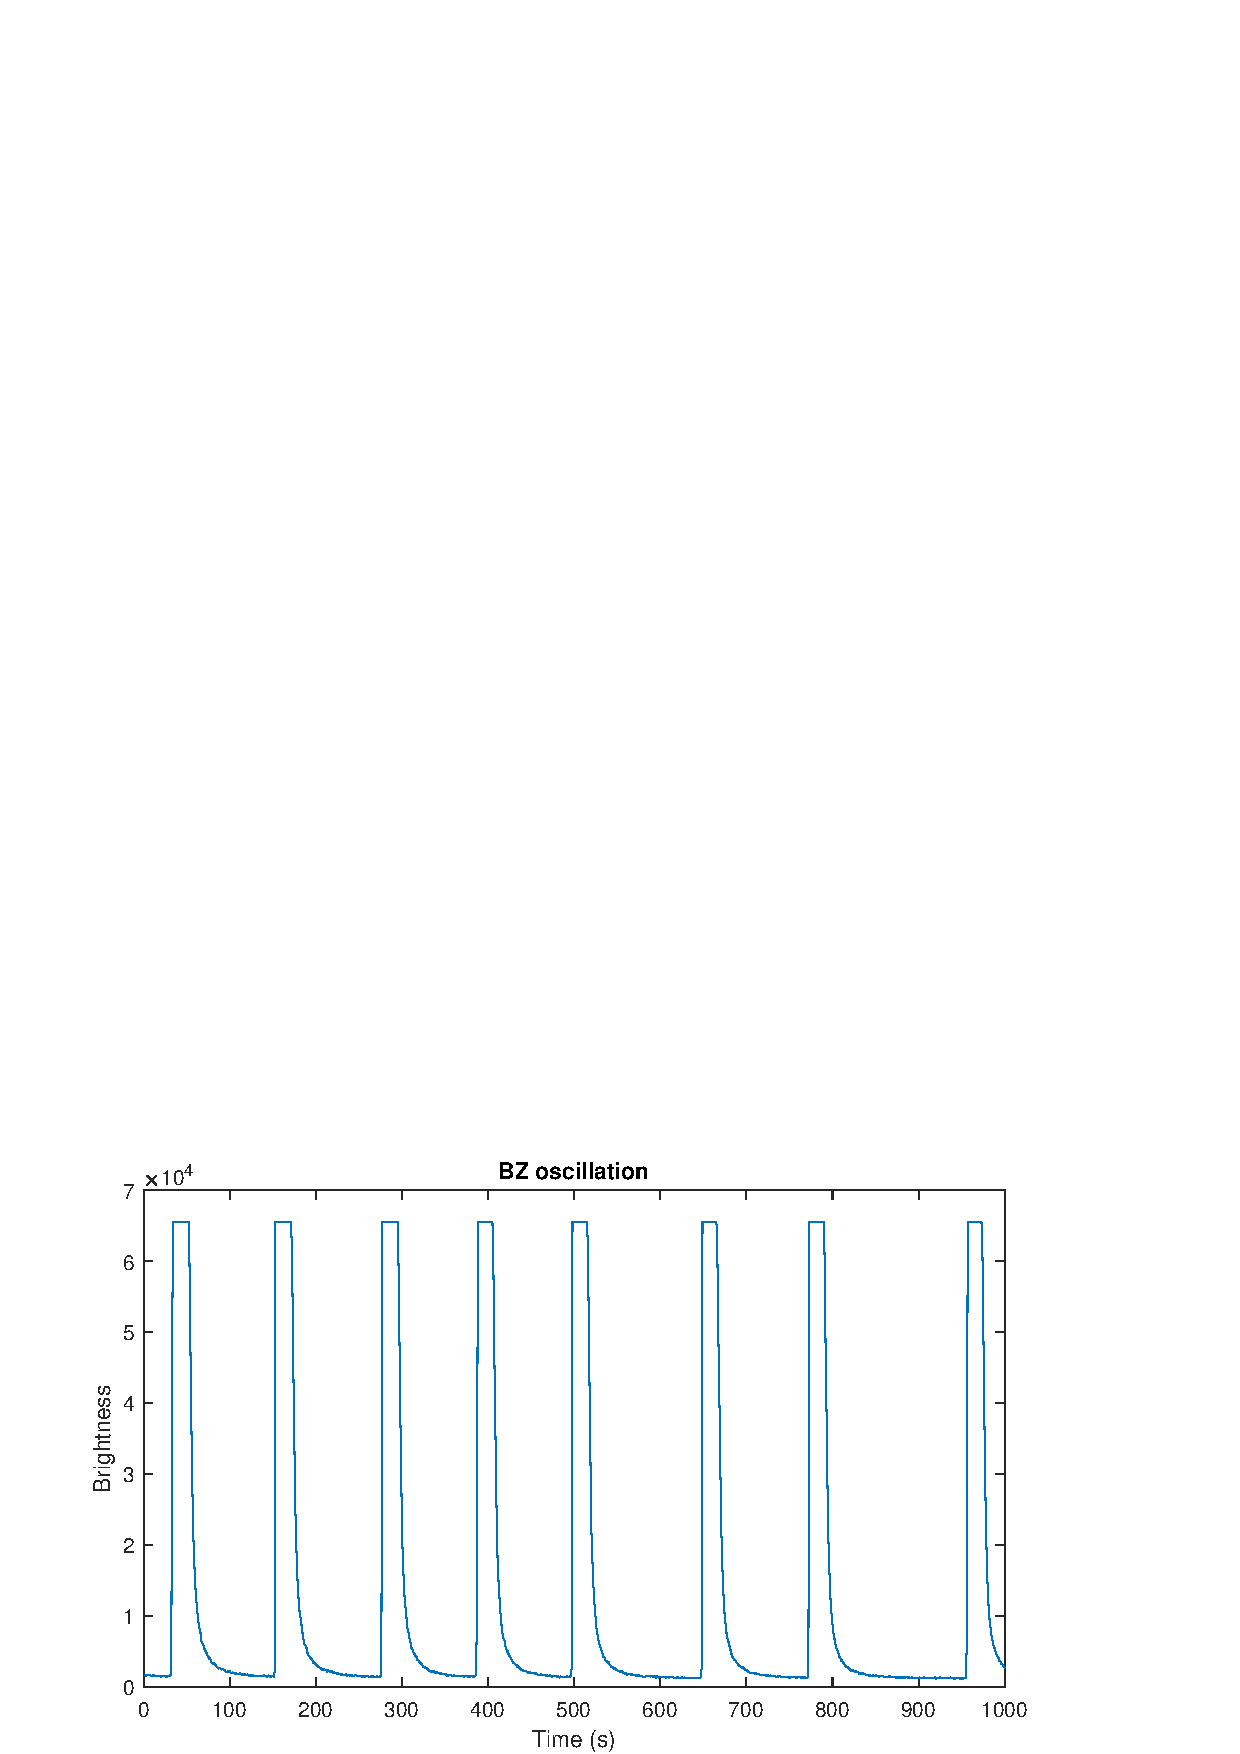
\includegraphics[scale=0.45]{osc-lab}
	\caption{Brightness of the solution in Figure \ref{fig:Osc} as a function of time. Notice that these oscillations do not occur with a constant period.}
	\label{fig:osc-time}
\end{figure}


BZ oscillations, on the one hand, occur when the reactants are constantly mixed in order to maintain uniform chemical concentrations throughout the medium in which the reaction takes place.  Figure \ref{fig:Osc} shows a flask containing the reaction at two different points in time, showing different brightnesses. Figure \ref{fig:osc-time} shows how the color of the solution (represented by its brightness) oscillates in time. We further notice that these oscillations occur at regular intervals, but are not strictly periodic. 


On the other hand, in the absence of vigorous stirring, diffusion becomes important, and the BZ reaction becomes an excitable, pattern-forming, \textit{reaction-diffusion system} and gives rise to \textit{chemical waves} \cite{ball1999self}. Unlike sound waves or electromagnetic radiation, however, chemical waves do not interfere the same way sound of electromagnetic waves do, i.e., they do not obey the principles of superposition.  Figure \ref{fig:Pattern} shows a typical pattern and how it evolves in time as propagating chemical waves. 


\begin{figure}[!htb]
	\centering
	\vspace{+15pt}
	\subfigure[]{
\includegraphics[scale=0.08]{pattern0}}
	\subfigure[]{
\includegraphics[scale=0.08]{pattern1}}
	\caption{Pattern formation due to the BZ reaction.}
	\label{fig:Pattern}
\end{figure}


It is fascinating and incredible how well a model as simple as the Oregonator could capture such complex behaviors. However, one must not to be too detached from the physical reality. Clearly, the predicted oscillations given by the model have well-defined periodicity and thus do not coincide with a true BZ oscillation, which is not strictly periodic (Figure \ref{fig:osc-time}). This is a reminder that in spite of the wonderful insights it has given, the Oregonator is still a much simplified description of a highly complex chemical interaction. 


\begin{acknowledgments}
I would like to thank Professor McCoy for introducing HQB to this topic, his guidance through this project, and the image data for the BZ reaction. I also thank Shannon Gray and Emily Padula for the helpful discussions and the original version of the BZ lab MATLAB code.  
\end{acknowledgments}


\bibliography{paper1}


\end{document}